\documentclass[11pt]{scrartcl}
\usepackage[sexy]{../../../evan}
\usepackage{graphicx}
\usepackage{float}
\usepackage{pgfplots}
\usepackage{subcaption}
\usepackage{filecontents}
\pgfplotsset{compat=1.18}
\definecolor{dg}{RGB}{2,101,15}
\newtheoremstyle{dotlessP}{}{}{}{}{\color{dg}\bfseries}{}{ }{}
\theoremstyle{dotlessP}
\newtheorem{property}[theorem]{Property}
\newtheoremstyle{dotlessN}{}{}{}{}{\color{teal}\bfseries}{}{ }{}
\theoremstyle{dotlessN}
\newtheorem{notation}[theorem]{Notation}
\newtheoremstyle{dotN}{}{}{}{}{\color{teal}\bfseries}{.}{ }{}
\theoremstyle{dotN}
\newtheorem{solution}{Solution}
\RequirePackage[linesnumbered,lined,boxed,commentsnumbered,noend]{algorithm2e}
\usepackage{algpseudocode}
% Shortcuts
\DeclarePairedDelimiter\ceil{\lceil}{\rceil} % ceil function
\DeclarePairedDelimiter\flr{\lfloor}{\rfloor} % floor function

\DeclarePairedDelimiter\paren{(}{)} % parenthesis

\newcommand{\df}{\displaystyle\frac} % displaystyle fraction
\newcommand{\qeq}{\overset{?}{=}} % questionable equality

\newcommand{\Mod}[1]{\;\mathrm{mod}\; #1} % modulo operator

\newcommand{\comp}{\circ} % composition

% Text Modifiers
\newcommand{\tbf}{\textbf}
\newcommand{\tit}{\textit}

% Sets
\DeclarePairedDelimiter\set{\{}{\}}
\newcommand{\unite}{\cup}
\newcommand{\inter}{\cap}

\newcommand{\reals}{\mathbb{R}} % real numbers: textbook is Z^+ and 0
\newcommand{\ints}{\mathbb{Z}}
\newcommand{\nats}{\mathbb{N}}
\newcommand{\complex}{\mathbb{C}}
\newcommand{\tots}{\mathbb{Q}}

\newcommand{\degree}{^\circ}

% Counting
\newcommand\perm[2][^n]{\prescript{#1\mkern-2.5mu}{}P_{#2}}
\newcommand\comb[2][^n]{\prescript{#1\mkern-0.5mu}{}C_{#2}}

% Relations
\newcommand{\rel}{\mathcal{R}} % relation

\setlength\parindent{0pt}

% Directed Graphs
\usetikzlibrary{arrows}
\usetikzlibrary{positioning,chains,fit,shapes,calc}

% Contradiction
\newcommand{\contradiction}{{\hbox{%
    \setbox0=\hbox{$\mkern-3mu\times\mkern-3mu$}%
    \setbox1=\hbox to0pt{\hss$\times$\hss}%
    \copy0\raisebox{0.5\wd0}{\copy1}\raisebox{-0.5\wd0}{\box1}\box0
}}}

% CS 
% NP
% Modulo without space
\newcommand{\nmod}[1]{\;\mathrm{mod}\;#1}
\newcommand{\np}{\texttt{NP}_\texttt{search}}
\newcommand{\p}{\texttt{P}_\texttt{search}}
\newcommand{\nph}{\texttt{NP}_\texttt{search}\text{-hard}}
\newcommand{\npc}{\texttt{NP}_\texttt{search}\text{-complete}}
\newcommand{\EXP}{\texttt{EXP}_\texttt{search}}
\newcommand{\xxhash}[2]{\rotatebox[origin=c]{#2}{$#1\parallel$}}

\title{CS 124: Data Structures and Algorithms}
\subtitle{Programming Set 3}
\author{Cao and Ziv}
\date{\today}
\newcommand{\courseNumber}{CS 124}
\newcommand{\courseName}{Data Structures and Algorithms}
\newcommand{\psetName}{ProgSet 3}
\newcommand{\dueDate}{Due: Thursday, April 18, 2024}
\newcommand{\name}{Denny Cao and Ossimi Ziv}
\renewcommand{\theques}{\thesection.\alph{ques}} % Change subtheo counter for alpha output
\declaretheorem[style=basehead,name=Answer,sibling=theorem]{ans}
\renewcommand{\theans}{\thesection.\alph{ans}}

% stuff for algorithm environment
%%% Coloring the comment as blue
\newcommand\mycommfont[1]{\footnotesize\ttfamily\textcolor{blue}{#1}}
\SetCommentSty{mycommfont}

\SetKwInput{KwInput}{Input}                % Set the Input
\SetKwInput{KwOutput}{Output}              % set the Output

\makeatletter
\newenvironment{compprob}[1][]
  {\renewcommand{\algorithmcfname}{Computational Problem}%
   \begin{algorithm}[#1]
   \long\def\@caption##1[##2]##3{%
     \par
     \begingroup\@parboxrestore
     \if@minipage\@setminipage\fi
     \normalsize \@makecaption{\AlCapSty{\AlCapFnt\algorithmcfname}}{\ignorespaces ##3}%
     \par\endgroup
   }}
  {\end{algorithm}}
\makeatother
%++++++++++++++++++++++++++++++++++++++++
% title stuff
\makeatletter
\renewcommand{\maketitle}{\bgroup\setlength{\parindent}{0pt}
    \begin{flushleft}
        {\Large\textbf{\@title}} \\ \vskip0.2cm
        \begingroup
            \fontsize{12pt}{12pt}\selectfont
            \courseNumber: \courseName 
        \endgroup \vskip0.3cm
        \dueDate \hfill\rlap{}\textbf{\name} \\ \vskip0.1cm
        \hrulefill
    \end{flushleft}\egroup 
}
\makeatother

\title{\psetName}
\begin{document}
\maketitle
\thispagestyle{plain}
\section{Number Partition}
\begin{compprob}[h]
        \SetKwInOut{Output}{Output~}
        \SetKwInOut{Input}{Input~}
		\Input{A sequence of $n$ numbers $A = \{a_1, a_2, \ldots, a_n\}$}
                        \Output{A sequence of $n$ numbers $S = \{s_1, s_2, \ldots, s_n\}$ of signs $s_i \in \set*{+1,
                            -1}$ such that the residual sum of the numbers in $A$ is minimized.}
                            \caption{Number Partition}
\end{compprob}
\begin{claim}
    \texttt{Number Partition} can be solved in pseudo-polynomial time. 
\end{claim}
\begin{proof}
   Suppose the sequence of terms in $A$ sum up to some number  $b$. Then each of the numbers in  $A$ has at most  $\log
   b$ bits. We will show there exists a dynamic programming algorithm that solves the \texttt{Number Partition} problem
   that takes time polynomial $nb$:
   \begin{itemize}
       \item \textbf{Subproblems:} Let $D[i,j]$ be whether it is possible for  $A[0,i]$ to sum up to $j$.
   
  \item \textbf{Recurrence:} The recurrence relation is given by:
    \[
   D[i,j] = (D[i-1,j+a_i] \lor D[i-1,|j-a_i|])  
   \] 
    Our recurrence is correct because if $D[i-1,j+a_i]$ is true, then we can subtract $a_i$ from $j + a_i$ (which is obtainable with the first $i-1$ elements) to get $j$. 
    Similarly, if $D[i-1,|j-a_i|]$ is true, then either we can add $a_i$ to the $j - a_i$ (which is obtainable with the first $i-1$ elements) to get $j$ or subtract $a_i - j$ (which is obtainable with the first $i-1$ elements) from $a_i$ to get $j$. 
    In doing so, we obtain every
    possible sum of the first $i$ elements of $A$. 

   \item\textbf{Topological Order:} We solve the subproblems in increasing order of $i$ and $j$.

    \item\textbf{Base Case:} $D[0,0] = \texttt{True}$ and $D[i,j] = \texttt{False}$ for all other $i,j$.

    \item\textbf{Original:} The original problem is to find the smallest $j$ such that $D[n,j]$ is true, or:
    \[
    \min \set*{j : D[n,j] == \texttt{True}, j \in [b]}
    \]

   \item \textbf{Time Complexity:} The time complexity of this algorithm is $O(nb)$. This is because for each
    subproblem we check if $b$ sums are possible (The maximum sum is $b$). When checking if a sum is possible, we
    take  $O(1)$ time to check 2 previous subproblems. Thus, the total time complexity is $O(nb)$ to fill the
    table. Iterating to find the smallest $j$ such that $D[n,j]$ is true takes $O(b)$ time. Therefore, the total time
    complexity is $O(nb) + O(b) = O(nb)$.
   \end{itemize}
    Therefore, the \texttt{Number Partition} problem can be solved in pseudo-polynomial time.
\end{proof}

\section{Karmarkar-Karp}
\begin{claim}
    \texttt{Karmarkar-Karp} can be implemented in $O(n\log n)$ time
\end{claim}
\begin{proof}
    The algorithm suggests that we are given a list of numbers, $A$, we select the two largest elements, $a_i$, and $a_j$, difference them, replace the larger of the two by the absolute value of their difference, and replace the smaller with 0. Repeat this until there is only one number left. To analyze the time complexity of a potential implementation, we can split the problem into steps:
    \begin{itemize}
        \item \textbf{Sorting}: To make it convenient to find the two largest elements, we can create a \texttt{max-heap}. Building this structure will take $O(n)$ time given that $A$ has $n$ elements.
        \item \textbf{Selecting}: Actually extracting the two largest elements involves running \texttt{extract-max} twice from our max-heap. Each of these extractions and restructuring of the heap afterwards will take $O(\log n)$ time.
        \item \textbf{Comparison}: Comparing the two values and computing their difference involves basic arithmetic and can be done in constant time given the problem definition. 
        \item \textbf{Inserting}: Inserting both the absolute value of the difference back into the heap takes $O(\log n)$ time. 
    \end{itemize}
    Every time we replace one of the elements with zeros, we are one step closer to the algorithm terminating, going from $n$ steps left to 1 step left. (given that it ends when the two max's are a number and zero). So the number of iterations of the [select, compare, insert loop] that we have to do is $n-1$. As a result, our time complexity is $O(n * (\log n + 1 + 1)) + O(n) = O(n\log n + n) + O(n) = O(n\log n)$.\\

    Therefore we have shown it is possible to implement the Karmarkar-Karp algorithm in $O(n \log n)$.
\end{proof}

\section{Using Karmarkar-Karp as a starting point}
Using KK as a starting point for the various random algorithms we get varying levels of improvement depending on the algorithm.
\begin{itemize}
    \item \textbf{Repeated Random}: using the starting point from KK in the repeated random algorithm will not necessarily have a big impact on its efficiency. Given that the algorithm randomly generates solutions anyway, any improvement will be a good improvement over the already good KK partition, but the random nature of the algorithm's selection would be equally likely to arrive to that bound anyway, so while the worst case scenario return is better from KK, there would be no other substantial improvement. 
    \item  \textbf{Hill Climbing}: This case is relatively similar to the previous. Setting KK as our starting point in Hill Climbing will definitely allow us to refine the solution further per the nature of the hill climbing algorithm selecting the best possible neighbor. That said, it will potentially trap us in a local minimum residue that isn't the global minimum. Even still, already having a strong starting point will provide a good jumping off point and any improvement will be even closer to ideal. Though when max-iter is very large, it may arrive at a similar, if not better solution regardless of starting point by continuously improving. 
    \item \textbf{Simulated Annealing}: KK will provide the most significant improvement here. Given the already strong solution from KK, the exploration involved in not picking an always better neighbor will allow for ideal use of this jumping off point. The original random starting point has a good chance to be too far away to explore ideal possibilities fully before temperature allows exploration. With KK's near-optimal residue, conditions are perfectly suited for the simulated annealing to explore neighboring solutions and quickly approach the minimum residue. 
    \item \textbf{Effect on Prepartition}: Using KK to start for the prepartition will create a binary assignment to two sign groups among which the elements will be split. This will create a $P$ array such that the numbers are all $1$ or $2$. Consequently, the selection of neighbors will vary than if we had pre-partitioned normally where the group assignment is variable $1...N$. The swaps would be between two selected sets of elements. This would put us closer to an ideal solution by the nature of the strong partitioning obtained by KK, making neighbor selection more efficient for pre-partitioned random algorithms. 
\end{itemize}
\section{Experimental Data}
\begin{table}[H]
   \centering
   \resizebox{\textwidth}{!}{%
   \begin{tabular}{c|c|c|c|c|c|c|c}
       Trial & KK & Repeated Random & Hill Climbing & Simulated Annealing & Repeated Random PP & Hill Climbing PP & Simulated Annealing PP \\
         \hline
            1 & 243525 & 365989989 & 130413807 & 820476299 & 721021115 & 1649 & 1193 \\
            2 & 75459 & 749147571 & 49649365 & 110886859 & 453801311 & 993 & 543 \\
            3 & 333585 & 60791321 & 592031675 & 410208631 & 382961939 & 103 & 95 \\
            4 & 364573 & 1019154041 & 525860527 & 559980607 & 572481879 & 2505 & 215 \\
            5 & 499274 & 1663890668 & 9600502 & 177089450 & 425379162 & 324 & 12 \\
            6 & 50679 & 983355655 & 61558941 & 91014911 & 483885527 & 537 & 619 \\
            7 & 6297 & 289923365 & 141851981 & 93675167 & 391212795 & 11 & 733 \\
            8 & 79255 & 52619949 & 41953499 & 186719479 & 530051507 & 611 & 115 \\
            9 & 17592 & 450914866 & 326632432 & 13836614 & 409700748 & 2032 & 538 \\
            10 & 46863 & 155134253 & 393724045 & 226479395 & 504317933 & 1009 & 1207 \\
            11 & 43178 & 334809164 & 208661436 & 297150226 & 309984058 & 2300 & 26 \\
            12 & 14289 & 95311037 & 106630491 & 525908655 & 311990773 & 145 & 319 \\
            13 & 7964 & 814199544 & 120018340 & 153072086 & 582754252 & 140 & 462 \\
            14 & 1084011 & 351859313 & 101787919 & 76680837 & 455126029 & 423 & 99 \\
            15 & 125164 & 503947338 & 301696718 & 733990202 & 517703010 & 54 & 522 \\
            16 & 111640 & 331168558 & 503991656 & 150497122 & 513564604 & 682 & 380 \\
            17 & 52602 & 250699462 & 10557910 & 833848632 & 279942744 & 1916 & 220 \\
            18 & 48789 & 1132800455 & 16538989 & 37511737 & 310552989 & 405 & 109 \\
            19 & 714008 & 370595408 & 45397324 & 211348136 & 604250196 & 118 & 882 \\
            20 & 104493 & 249088631 & 111054379 & 55343659 & 502681395 & 923 & 533 \\
            21 & 1528478 & 238734766 & 195013800 & 568113386 & 450889340 & 1178 & 432 \\
            22 & 26423 & 422879069 & 146569383 & 939114721 & 543061263 & 145 & 123 \\
            23 & 145283 & 1236219271 & 55103153 & 221245635 & 418310477 & 511 & 161 \\
            24 & 13428 & 168078920 & 466859430 & 268728928 & 378196608 & 368 & 330 \\
            25 & 25127 & 449412203 & 410386189 & 466687861 & 681660055 & 487 & 113 \\
            26 & 118098 & 250827774 & 42106260 & 37768412 & 314325108 & 922 & 154 \\
            27 & 620257 & 191868027 & 106642211 & 109380535 & 778808941 & 1271 & 113 \\
            28 & 174312 & 51826154 & 33569164 & 206867538 & 492283932 & 2068 & 584 \\
            29 & 369267 & 940519427 & 591488585 & 215969543 & 395210615 & 1737 & 17 \\
            30 & 34617 & 30235707 & 82435633 & 52819311 & 454803825 & 369 & 889 \\
            31 & 79954 & 460060798 & 498708382 & 442097596 & 387721818 & 156 & 582 \\
            32 & 102734 & 71237852 & 111295898 & 651610774 & 399201556 & 1824 & 70 \\
            33 & 56344 & 296305734 & 233808082 & 33672900 & 760619780 & 1442 & 84 \\
            34 & 67309 & 206556833 & 386724715 & 115222913 & 368287833 & 2389 & 103 \\
            35 & 136493 & 538893389 & 52846929 & 67880597 & 390770209 & 43 & 535 \\
            36 & 330164 & 39215638 & 610324334 & 716191394 & 333574470 & 32 & 76 \\
            37 & 142413 & 262801565 & 126215233 & 285896785 & 1089348671 & 719 & 25 \\
            38 & 191694 & 51841656 & 6374792 & 352337616 & 506461030 & 614 & 118 \\
            39 & 133514 & 142928562 & 389524862 & 134834086 & 380314252 & 424 & 132 \\
            40 & 186766 & 460056552 & 1010404346 & 233133226 & 424693488 & 28 & 112 \\
            41 & 9981 & 352892269 & 33401523 & 773077949 & 400312089 & 109 & 261 \\
            42 & 271 & 26638341 & 121317129 & 2258165 & 487764263 & 1567 & 323 \\
            43 & 328860 & 259517152 & 323308008 & 514894280 & 352148016 & 366 & 10 \\
            44 & 488087 & 75670641 & 155951977 & 290257285 & 275895987 & 2027 & 413 \\
            45 & 20099 & 97684499 & 8263465 & 67611609 & 502274553 & 129 & 195 \\
            46 & 152253 & 84980193 & 1105069359 & 806007089 & 538698021 & 1391 & 127 \\
            47 & 25640 & 546039342 & 43459306 & 559689932 & 639759114 & 206 & 186 \\
            48 & 3313304 & 26877136 & 544196480 & 1421963684 & 388432910 & 698 & 48 \\
            49 & 290118 & 113329412 & 91852728 & 260402170 & 512143770 & 334 & 222 \\
            50 & 102994 & 209427994 & 91332756 & 1995555168 & 359393702 & 690 & 58 \\
            Average & 264750.44 & 370579149.3 & 239754098.3 & 371540195.8	& 473374593.2 &	822.48 &	308.36
    \end{tabular}}
    \caption{Experimental Data}
\end{table}
% Scatter plot of the data, log scale for y axis different colors for each algorithm
\begin{figure}[H]
    \centering
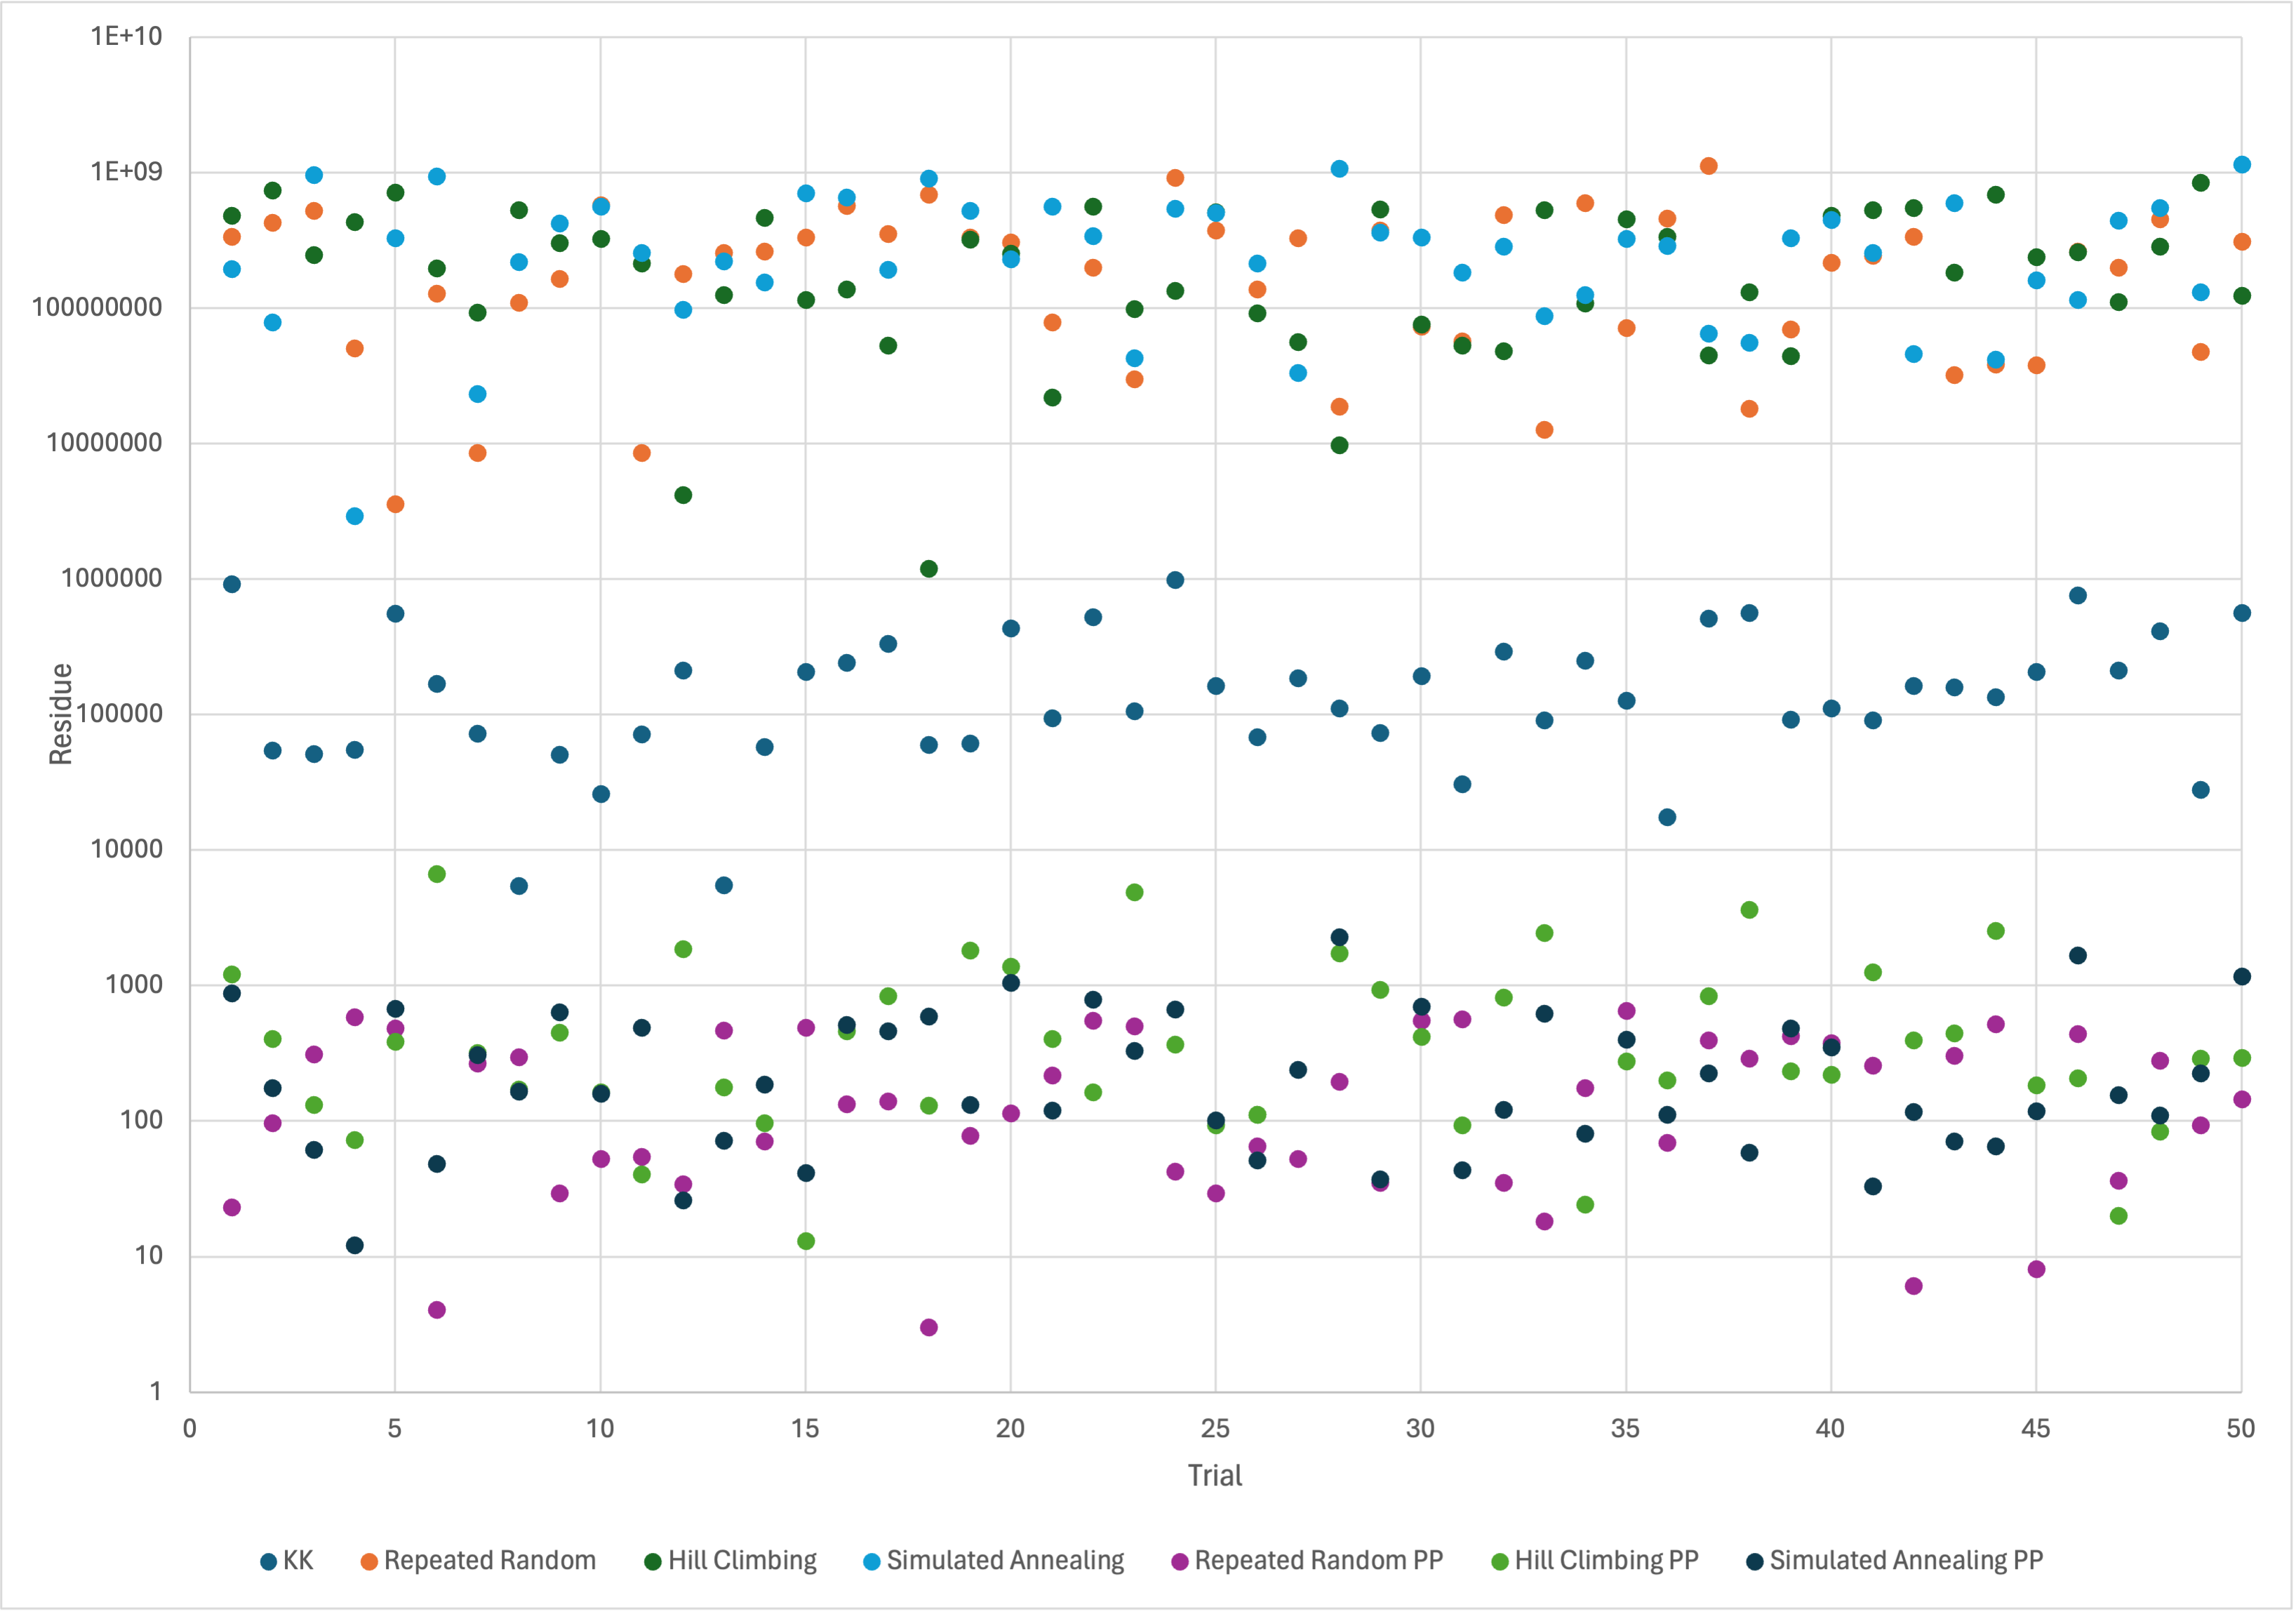
\includegraphics[width=\textwidth]{data.png}
\caption{Scatter Plot of Experimental Data}
\end{figure}
We notice that there are 3 distinct ``areas'' created by the different algorithms defined by whether they used
standard or prepartitioned solutions with the latter producing the best results and the former producing the
worst, bounding the middle ground of Karman-Karp. 
\end{document}
